\chapter{Remix Culture}
\label{ch:ch1_RemixCulture}

% --- Chapter 1 start ---

Remix Culture is the overarching theme of this dissertation. This phenomenon encompasses a large number of domains and aspects of everyday life involving creativity, thus shaping the way these works are being created, shared, used, and reused. Indeed, the fruition and the reuse are the most characterising facets of the Remix concept.

As mentioned in the introduction, Remix Culture is a transformative practice. By taking one or more pieces of existing items – both physical and digital – new works can be created. For instance, the replacement of an audio source within a certain video or more complex arrangements like entire movies made by using other audio visual elements are both valid examples of transformative practices. These kinds of remixes can radically change the meaning and the cultural perception of the original works.

It appears that the Remix Culture can be seen from two high-level perspectives, the first tied to the digital evolution. Indeed, among the inspirations of the Remix Culture is the Free and Open Source-Software (“FOSS”), an initiative which will be introduced in paragraph \ref{sec:IPR} \emph{Open Source} as a precursor to the Open Source movement. In short, the goals and ideas of these movements are mainly oriented towards encouraging a “free” distribution of software. “Free” is a vague term that will have to be discussed later in more details.

A second perspective is not exclusively tied to the digital evolution, rather it can be seen as a sociocultural concept that affects several aspects of human behaviour. From a broader perspective, the Remix Culture can be thought of as a way the society works and evolves through history. The idea can be explained by using the popular metaphor of “standing on the shoulders of giants” in the sense used and intended by Isaac Newton\footfullcite{bbcNewton}. Therefore, the ability to discover and enhance knowledge – hence progress as humans – can be reached thanks to the contributions of past and present human generations with the knowledge that had been passed to us.

This concept is further sustained by Lev Manovich in his article “Remixing and Remixability”\footfullcite{ManovichRemixability}. The author argues that:

\begin{displayquote}
    “most human cultures developed by borrowing and reworking forms and styles from other cultures; the resulting “remixes” were to be incorporated into other cultures. Ancient Rome remixed Ancient Greece; Renaissance remixed antiquity; nineteenth century European architecture remixed many historical periods including the Renaissance…”.
\end{displayquote}

This excerpt suggests a definition of remixability as a common trait of human behaviour as deducted from a historical perspective. This can be generalised to humans as communities\footfullcite{wikiSenseOfCommunity}, as well as individuals. The latter view becomes the core point of author’s subsequent analysis when describing the modern times. The core point of his argumentation is the major novelty introduced by the Internet, that is the unprecedented level of participation of individuals with the relative ease of accessibility. Indeed, related to this aspect, he states that “culture has always been about remixability, but now this remixability is available to all participants of Internet culture”\footfullcite{ManovichRemixability}. Nowadays, the pervasiveness of Internet connectivity has led to a professionalization of individuals. Thanks to information available on the web combined with software tools that allow to produce new content, the individuals can become active members of the Remix Culture. Finally, acting as creators, members of the public are able to share their work almost instantly, everywhere and at little or no cost. 

As a matter of fact, this reflects the tendency of new social interactions enabled by the Internet. Many of the most popular online platforms, like Youtube, TikTok, Instagram, etc. make extensive use of the Remix Culture. In the next section \ref{sec:RmxExamples} \emph{Examples of Remixes}, some practical examples of remixes from various disciplines and time frames, ranging from texts, music, films to videogames will be presented to better illustrate the whole phenomenon.

Before expanding further in framing Remix Culture, a first glance on common issues can be taken by reflecting upon this rather radical change of paradigm. Hence, the change from an analogic and physical to a digital environment. It could be argued that the national and international laws have not responded adequately to this change of paradigm. According to Lawrence Lessig, who may be considered among the most prominent figures in favour of this argument, states that: 

\begin{displayquote}

“For the first time, the [copyright] law regulates ordinary citizens generally. For the first time, it reaches beyond the professional to control the amateur— to subject the amateur to a control by the law that the law historically reserved to professionals.”\footfullcite{LessigRemixMA}

\end{displayquote}

This suggests an underlying problem from a legislative perspective, thereby the copyright law. Further evidence will be provided in paragraph \ref{sec:IPR} Intellectual Property Laws and Reusability. The overall point is that by analysing the past and current evolution of works of creativity made by “amateurs” i.e., general public, it seems that the law has taken some stringent measures to limit the Remix phenomenon. This is also true for professionals and large businesses. Additionally, some uncoordinated decisions have been made to respond to certain issues with the practical applications of copyright laws. This overall might be considered as an inhibitory factor acting against the Remix Culture ideas and practical applications.

Another interesting point of view related to the concept of Remix Culture is given by the aforementioned Lawrence Lessig, the founder of Creative Commons. In his book “Remix Making Art and Commerce Thrive” he defines Remix Culture as a Read/Write (“RW”) culture as opposed to a Read/Only (“RO”) culture. The author uses an analogy of how popular computer systems work (for example Linux based systems, Windows etc). Basically, users with read and write permission on a file or directory are authorized to read it and make changes. On the contrary, the read only permission allows only for files and directories to be read disabling the ability of making any modifications.

Returning to the cultural context, the latter is the situation where the users or the general public passively consume the content made by someone else. This is frequently the case of professionally made content, backed by expensive tools and potentially complex organisational structures. For example, the TV broadcasts, production of high budget movies and their subsequent distribution on CDs, DVDs, etc. It could be argued that the Read/Only culture lasted until the times of Internet pervasiveness, as it is characterised by a top-down consumption of cultural objects. On the other hand, the Read/Write culture allows for a democratized participation on the creative process. Hence, a democratization of the act of creativity where people participate in the creation and the re-creation of culture.
These arguments represent a paradigm switch. In the Read/Only culture information flows one-way – unidirectionally –, while in the Read/Write culture the information is multi directional or, speaking in terms of networking: peer to peer like\footfullcite{wikiPeerToPeer}.

At this point, it should be clear that the technological progress allowed to minimize the gap between the professionally created content and the works of creativity that can be made without substantial investments or infrastructure. This can be accomplished thanks to software that makes the technical operation of “remixing” relatively easy.

This concept is also exemplified by Lev Manovich in relation to music remixes and music mashups. In his article “Remix and remixability” he states that: “Although precedents of remixing in music can be found earlier, it was the introduction of multi-track mixers that made remixing a standard practice" \footfullcite{ManovichRemixability}\,\footnote{This specific example is somewhat related to this dissertation’s practical application. Instead of music as exemplified by Lev Manovich any type of media can be put into a multi-track editor to create new remixes.}.

Hence, what really made the Read/Write culture come to life was the 21st century digital revolution. Indeed, there are some relevant differences between the way things could be created, re-used, and shared before the age of Internet. A notable example showing these differences is the invention of the mechanical movable-type printing press, that is an efficient machine for printing texts. The main difference between the printing press and the Internet is that the printed output copies were inferior to the originals in terms of quality. The affordability was also an issue, costs related to printing a copy prevented people to fully benefit of that invention. Another aspect of this problem is that people had little choice regarding the production of copies for themselves. The alternative choices – until the introduction of low-cost home prints – would imply an inferior quality to those coming from the professional printing businesses. Thus, the whole process relied on professionals.
On the other side, the Internet can be seen as the most efficient, low-cost copying and sharing mechanism accessible from everywhere. Furthermore, the sharing process allows for resources to be distributed globally between connected users, and this is a substantial difference from the previous models. Therefore, users do not often need to rely on professionals to make creative works.

These differences can be further explained from an economical perspective as the distinction between rival goods and non-rival goods\footfullcite{wikiRivalry}. In general, most physical goods are rival goods. For example, a sandwich is a rival good, because the act of eating it clearly diminishes its value. A sandwich loses its value while it is being eaten, so to speak. Sharing rival goods implies the that the benefits of use are decreased or eliminated, so sharing a piece of sandwich produces a tangible loss for the owner of the sandwich. Analogously, sharing a printed copy of a book is an example of rivalry because it prevents the original owner from its unlimited consumption.

On the other side the definition of non-rival goods implies that: “… one person’s enjoyment of a good does not diminish the ability of other people to enjoy the same good.” \footfullcite{KotchenPublicGoods}. Hence, ideas and words tend to be non-rival. Sharing them does not make them worse or less valuable. An exception of a physical good that is non-rival could be a public bench. The bench value is not significantly diminished when used by people (at least, hopefully, if it is being used correctly). From this perspective a large majority of digital goods are non-rival. A relevant example is an e-book, no one ever “bought” an e-book, people buy a license to read e-books on their devices of choice. Namely, the use of copies does not preclude its accessibility from others and is not directly connected to tangible losses. A few exceptions like domain names and so on exist in this category as well.

Expanding upon the non-rivalry definition, in his book “The Success of Open Source (2004), Steve Weber argued that some ideas, words, etc. are definable as “anti-rival goods” meaning that they are improved by being shared in a manner similar to the economics idea of the “Network effect”\footfullcite{wikiNetworkEffect}. Some examples could be the case where a social media gets more powerful as more and more people are using it, or an article becomes more valuable as its hyperlink is being shared across the web, etc. In short, the act of sharing increases the benefits for other participants. For this same reason it could be argued that the efforts to combat climate change are non-rival because the benefits of these actions are shared among all the word’s living species, including for example all the nations who refuse to do so. 

This final point of analysis suggests that the Remix Culture could be in fact non-rival. This argument could be rephrased as a direct question, “are the works of creativity produced as a result of remixing beneficial for the general public?”

Unfortunately, the proposed answer is murky, since from a general point of view it would be very hard to answer with a simple “no” or “yes”. It might be argued that it depends on case to case and on the relative contexts where this question is made. Probably, the answer might not always be positive from the perspective of original creators or de facto owners of works whom creations might be used in a way that contradicts their believes, such as propaganda, commercial profits, etc. Nevertheless, the key point worth considering is that as a matter of fact, everything can be remixed and distributed globally.

In this view, a consideration on the PH-Remix project case is pertinent. Among the project’s goals are dissemination, discovery, use and re-use which may enhance the value of created content. From a practical point of view, short clips are extracted from films uploaded to the platform – mainly documentaries at the time of writing – using Artificial Intelligence algorithms. Subsequently, in an idealistic scenario all the clips should become available for remixing i.e., being arranged and combined with other clips to form new audio-visual creations.

However, the tendency of the film industry could be considered sceptical about these ideas or simply not fully aware about the possibilities and new ways of innovating provided by digitisation. Considering the nature of the content initially put on the platform, it could be argued that cultural heritage works and especially documentaries should oblige a moral and ethical motivation of giving back to the communities and not be closed in organisational siloes protected by stringent laws. Indeed, PH-Remix for cultural heritage would be a case of non-rivalry because it should be desired to share the messages and stimulate a debate with as many people as possible with as little limits as possible.

Naturally, critiques about the idea of Remix Culture exist\footfullcite{rmxWoRomance}. They will be further discussed in the next paragraph in relation to copyright issues. It could be argued that a relevant part of human progress alongside with some of the most iconic inventions were made thanks to the presence of copyright laws. Nowadays, by taking into consideration that the cost of distributing content is as low or almost nonexistent for digital goods it may still be necessary to reward the creators of intellectual property.

This objectively seems to be true. Remix culture can be enabled by openness and open source licenses, but these are not a silver bullet for all projects and creations. A relevant example was once provided during the “Open Cultures” course at King’s College London by Dr John Lavagnino. He argued that J.K. Rowling could probably not have finished the Harry Potter books if she had decided to start publishing them without a license. A source of income is often needed and necessary. On the other hand, the more people who read Harry Potter the better. Generally, as a creator you probably would want to get as many people as possible to watch/be able to consult your creation. In chapter \ref{ch:ch2_ProjectManagement} \emph{Project management in interdisciplinary projects}, arguments advocating for a sustainable economy for content creation – especially for cultural heritage – will be discussed in more detail. 

\section{Examples of Remixes}
\label{sec:RmxExamples}


The practice of modifying both physical and digital items has a long-standing tradition. Remix applies to music, movies, cooking recipes, software, and many other disciplines. After introducing the Remix Culture mainly from a theoretical point of view, it is useful to make some practical examples to better understand the overall concept. For this reason, a selected list of examples from different domains – although mainly focused on the modern age time frame – is presented in this section.

An in-depth study of the creative processes and the way content is being re-used was done by Kirby Ferguson in his four-part video series titled “Everything is a Remix”\footfullcite{everythingIsARemix}. Indeed, he states that the acts of copying, transforming, and combining are the basic elements applicable at any level of creativity. Hence, the following assertion: “creativity is not magic, it happens by applying ordinary tools of thought to existing materials”\footfullcite{everythingIsARemix3}.

Music mashups are one of the most common examples of such transformations. Specifically, hip hop music was one of the first musical forms to incorporate samplings in the recordings\footfullcite{wikiMashup}. Thereby, the results are creative works which typically incorporate fragments of other songs. These fragments are generally re-arranged, thus transformed to produce new sounds and songs. Indeed, in most cases mashups are legal by considering them under the various boundaries of “fair use” law doctrine. These boundaries are usually fuzzy although the tendency of re-using pieces of other songs is very popular among many artists.

One example of a band which crossed boundaries of fair use is Led Zeppelin. They copied significant part of other songs without making fundamental changes. Two documented examples of songs subject to legal claims can be seen on the list below:

\begin{itemize}
\item Led Zeppelin song: “Bring it on home” was a copy of Willie Dixon – “Bring It On Home”\footfullcite{ledZeppelin1}
\item Led Zeppelin – “Stairway to Heaven” most likely copied from the band Spirit with their song “Taurus”\footfullcite{ledZeppelin2}
\end{itemize}

Another discipline which makes extensive use of Remix is the cinema industry. Many movies are inspired by the surrounding works of culture. Nowadays, a common technique consists in transforming the “old” into the “new”. That means taking or re-creating already existing materials from literature, actual events, etc. and producing movies for the current generations. Even existing movies are often a base for new cinema adaptations and frequent prequels and sequels.

One important example of remixing in the film industry are the Disney movies. The Walt Disney Company made extensive use of works from the public domain. Some examples from their repertoire of animated films history are listed below:

\begin{itemize}
\item The Little Mermaid is based on the “The Little Mermaid” fairy tale written by Hans Christian Andersen.
\item Alice in Wonderland is based on the novel “Alice's Adventures in Wonderland” and its sequel, “Through the Looking-Glass” both authored by Lewis Carroll.
\item Aladdin is based on the folk tale “Aladdin from the Arabian Nights” originated from the Middle Eastern culture and later interpreted by Antoine Galland.
\item Mulan is based on the traditional Chinese story of “Hua Mulan”, a legendary folk heroine. 
\end{itemize}

Once transformed into animated movies, Disney likewise any other film producer, were entitled to a period of exclusivity on their productions thanks to copyright. Then after a certain period their work is supposed to enter the public domain to be freely used and built upon. This case was regulated by the American legislation in the Copyright Act of 1976\footfullcite{wikiUSCopyrigh1976} which established the duration of copyright for the life of the author plus 50 years, or 75 years for a work of corporate authorship.

Interestingly, some companies and prominently Disney lobbied to have their terms of copyright extended\footfullcite{wikiUSCopyrighExtensionAct} with the Copyright Term Extension Act, also known as “Mickey Mouse Protection Act”. The company decided to prevent others from copying its works. Therefore, standing to the current copyright terms, Mickey Mouse, which firstly appeared in 1928, will enter the public domain starting from 1st January 2024\footfullcite{mickeyMouse}. It could be argued that by trying to foresee into the future, Disney will attempt to prevent it from happening by using other laws including trademark protection and using precedents in their favour from other court verdicts.

Returning to the practical cases, the film industry is a rich source of similar examples. For instance, an in-depth analysis of the Star Wars series results in finding multiple references and inspirations from historical events, fiction literature, etc. as well as some copied elements from other film productions. It could be argued that without the influence of past creations Start Wars would not have been created.

The digital evolution alongside with the birth of software for video editing allowed for a more accessible and complex remixing of new content outside of the professional world. Fan-made trailers, remixes, memes that spread virally are all consequences of the ease of use enabled by a mix of modern technology combined with user’s creativity.

Certainly, a long list of important examples could follow. For example, Machinima\footfullcite{machinima} productions, videos generated from video games graphic engines are a relevant contribution to re-use.
The core point is that the strength of these creations is also traceable to the communities of users that participate in the creative process and the consumption. Indeed, there are several examples of Remixes as community efforts.

Perhaps the most well-known and successful community effort is Wikipedia. Wikipedia’s main power is a huge community of active volunteers thanks to which it was able to succeed.

Other projects like Free Beer\footfullcite{freeBeer} and OpenCola\footfullcite{openCola} are examples of remixing in the physical world. They respectively consist in creating and improving recipes for beer and (coca) cola and encouraging their production by adopting a permissive license to the recipes.
In reality, the latter example is connected to the Open Source community as an attempt to replicate the concepts of free sharing and contributing into the physical world which was already a common practice in the software world. 

Naturally, Remix could be viewed as a form of art. Like the latter it is also subject to personal interpretation because, among its goals, is the creation of spaces for debate. Obviously, they often might be a source of tensions and critiques, as the example below.


\begin{figure}[H]
\centering
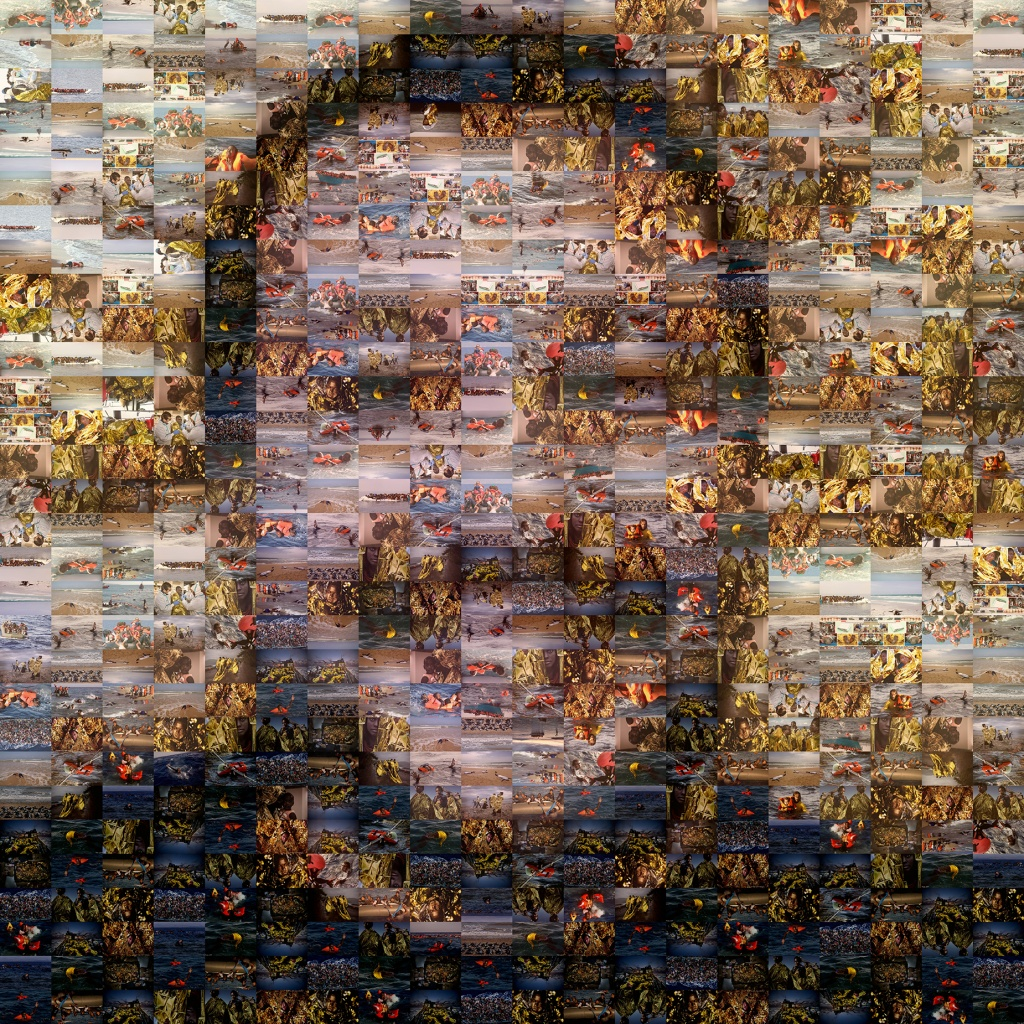
\includegraphics[width=0.6\textwidth]{images/arteAcquaSalvini.jpg}
\caption{"Arte dell'acqua" by students of Russoli High School (Pisa)}
\label{fig:arteAcqua}
\end{figure}

Figure \ref{fig:arteAcqua} "Arte dell'acqua" is a collage of approximately 400 photos of migrants which depict some tragedies happening at sea while trying to reach the coast. Together the pictures form the face of an Italian politician, Matteo Salvini. He is known for his ideological line against illegal immigration as he advocates for stronger actions and policies to enforce its prevention. Indeed, these forms of remixes can inevitably create controversies. Nevertheless, art encourages reflection and debate and above all it is an expression of free speech.

Lastly, copying is not necessarily equivalent to plagiarism. For instance, this whole dissertation could be seen as a remix. Originated by combining and arranging a set of factual sources with quotations alongside with the author’s academical background, personal experiences, and cultural bias to produce something new. 
While this last example of remix is perfectly legal – if it complies with some rules about academical quotations, etc. – and thus cannot be considered as a plagiarism, the same cannot be said about other contexts and media types.


\section{Intellectual Property Laws and Reusability}
\label{sec:IPR}

Understanding the concepts related to intellectual property (“IP”) and how they are regulated, is fundamental in order to acquire a complete picture of the Remix Culture.

Naturally, the activity of Remix is deeply interconnected with a multitude of laws. It is fair to debunk upfront that an extensive analysis of the topics presented in this section is beyond the scope of this work.  These are complex topics where legal terms involve the use of legal technicalities which differ from country to country. However, understanding the fundamentals of concepts like copyright and licensing is fundamental to explain and to illustrate some frequent problems occurring when adopting the Remix Culture.

As introduced in the previous paragraph, the re-use of content can be substantially limited and potentially discouraged because of the legal bounds applicable to a multitude of physical and digital goods. These legal bounds are typically expressed in form of author’s rights – or copyright, as these terms are used interchangeably in this dissertation – and can be contained in licences applicable to different kinds of works. In short, by creating new works authors are automatically entitled to exclusive rights on them and, as long as a permissive license is not applied, these works cannot be freely reused by others.

In reality, this might often work as a chilling effect, that is, “a discouraging or deterring effect, especially one resulting from a restrictive law or regulation” \footfullcite{collinsChillingEffect}. Furthermore, this effect can also be attributed to the quantity and the complexity of regulations affecting the specific items that might be of interest for re-use. A relevant argument in favour of this assertion comes from a phenomenon called proliferation of licenses\footfullcite{wikiLicenseProliferation}. This is originated from the creation of a large number of similar agreements that might require some domain specific knowledge for their interpretation. Additionally, licenses – whose main goal is to clearly explain the rights and limitations applied to a specific object – are often incompatible between each other, even if they are similar in their permissiveness or strictness.

The subsequent analysis will be focused on illustrating an overview and developing an understanding of the legislative implications of some legal terms that are relevant for the Remix Culture.

Firstly, “Intellectual Property Rights” (“IPR”) is an umbrella term for a category of rights which regulate intangible creations of the human intellect\footfullcite{forbesIPR}.

\begin{displayquote}
“The main purpose of intellectual property law is to encourage the creation of a wide variety of intellectual goods. To achieve this, the law gives people and businesses property rights to the information and intellectual goods they create, usually for a limited period of time.”\footfullcite{IPRightUses}
\end{displayquote}

As seen in the above explanation, the reason for restricting the IPR duration to a limited period of time is mainly motivated by the goal of encouraging further creations. Hence, during the time of “exclusiveness”, authors can earn profit which in turn acts as an economic incentive for creation in the first place.

Secondly, speaking purely in terms of IPR might be considered as an overgeneralization. Richard M. Stallman argues that including different sets of laws under the IPR term is misleading\footfullcite{IPRGNU}. The former frequently happens with within the language of news media. Nevertheless, the subject’s literature about IPR commonly includes a number of typologies of intellectual property belonging to different branches of law. Namely, rights, patents, copyright, industrial design rights, trademarks, registered designs, trade secrets and so on, also depending on the jurisdiction.

As introduced in the previous paragraph, Remix Culture could potentially be influenced by all of these laws. By taking into consideration the most common use cases a subset of IPR typologies can be taken for a deeper analysis. Specifically:

\begin{itemize}
\item Patents
\item Trademarks
\item Copyrights 
\end{itemize}

Patents are used for protecting inventions. Namely, creativity works that are new, not trivial (for experts in the subject/domain) and are useful, thus capable of being used in some kind of industry. Patents give their owners the right to prevent others from making, using, selling an invention without an explicit permission. For example, scientific or mathematical discoveries cannot be patented, as well as a literary, dramatic, musical, or artistic work and many others. On the other side new plant varieties, medicines, machines, innovative solutions to technological problems are generally valid targets for patents.
An ongoing debate regards the creation of software. The European legislation regulated by the European Patent Convention explicitly excludes the possibility of patenting “computer programs” as stated in Article 52 “Patentable inventions"\footfullcite{EPC}. Still, it is subject to interpretation by courts. Vice versa the American legislation tend to allow software patents.

Certainly, from the point of view of the Remix Culture, software patents could have long-term negative effects. Namely, as stated by the Free Software Foundation Europe, “they specifically inhibit the development of useful software by blocking compatibility and interoperability“\footfullcite{fsfe}.

Secondly, trademarks are some sort of signs that distinguish a company or a service from another. They are also frequently used for marketing purposes like branding, product recognition, etc. Logotypes are a classical example of a trademark. For instance, the Nike “swoosh”, the Apple “bitten apple” and McDonalds “golden arches” are among the popular examples of trademarks.

Finally, copyrights regulate that works cannot be copied without the explicit owner’s permission. This applies to any medium. For example, nobody can make a movie based on a book without obtaining the permission of the owner of the book copyright. Copyright can protect literary works, including novels, instruction manuals, computer programs, song lyrics, newspaper articles, and some types of databases. Perhaps the most important characteristic of copyright is that it does not have to be applied for. Everyone gets it even if not aware of it.

These three are just some selected examples that creators should be aware of when doing remixes. Interestingly, it seems that the just introduced concepts are similar between the physical word and the digital world. Therefore, it could be argued that they are a straightforward translation of legislative terms originated from the history rather than new concepts adapted for the 21st century. This can be explained by considering that the technological progress happened very fast and especially the Internet was an abrupt revolution. In his article “The fight to keep ideas open to all” James Boyle, professor of Law at Duke University, analyses the current restrictions of IPR in a digital environment. He also states that:

\begin{displayquote}
“The internet has dramatically lowered the cost of copying, including illicit copying. When the web was first weaved in the 1990s, intellectual-property owners found their property had, involuntarily, been turned into a common. Strong new copyright rules and draconian enforcement seemed to be necessary to tame the rebellious digital commoners and reclaim the level of control that had existed in an analogue world.”\footfullcite{economyst}
\end{displayquote}

As seen in the above quotation, there are aspects that may justify some actions and fears of the copyright holders. In the recent years, policymakers, faced by arguments and lobbying, decided to adopt, and extend a copyright model which currently may seem as more and more unfit for the technological progress.

Nowadays, this led to a growing quantity of issues. In the same article James Boyle affirms that our smartphones are covered by between 5,000 to 15,000 patents and up to 250,000 if considering all the related patents. The general idea of scholars and professionals advocating for a more liberal approach to digital right is that intellectual property in the actual form blocks innovation and can be harmful for the society.

An example, relevant especially at the time of writing, might regard life-saving creations like vaccines\footfullcite{CCcovid19}. As finally stated by Boyle: “In medicine, rafts of patents obstruct research into treatments such as a malaria vaccine; the costs of just identifying the relevant patents is [sic] prohibitive. Such a system is great for patent lawyers, whom I train. It is unlikely to be good for society as a whole.”\footfullcite{economyst}\,\footfullcite{AcadTimesMalaria}

Returning to the digital objects, the copyright laws evolved in terms of their enforcement. Indeed, they can also be efficiently prosecuted – although sometimes wrongly, by using technology. A relevant example is the YouTube Content ID software\footfullcite{GoogleYTID} which automatically checks for the presence of copyrighted materials. This happens when users upload their media to the YouTube platform.

\begin{displayquote}
“The software establishes a link between an existing work and an uploaded work such as a remix. If the content matches, the video may be automatically blocked, or the sound muted, and the user is automatically informed by e-mail that the material has been disabled”.\footfullcite{wipo2015}
\end{displayquote}

From this perspective, it might be deducted that a potentially dangerous direction would consist in maintaining the current state of IPR and enforcing it through the use of technology. This could be especially harmful for the Remix Culture phenomenon.

\subsection{Derivative Works and Fair Use}

As introduced in the previous section, the Remix Culture often faces problems regarding the legal bounds. Namely, the Intellectual Property Rights. On the other hand, the law also imposes rules and exceptions under which legal works can be created. Specifically, the concepts of derivative works and fair use are key for limiting the application extent of IPR.
In the practical applications of remixes, it seems that a common source of problems derives from how contents coming from a variety of sources are used and distributed for the creation of new works. Indeed, this discourse could be framed into the legal perspective by using the term of “derivative work”. By considering the definition from the Merriam Webster legal dictionary, a derivative work is defined as a “a piece of intellectual property that substantially derives from an underlying work”\footfullcite{merriamWebsterDerivativeW}.

From a general perspective, the notion of derivative works seems to be consistent across many national and international legal systems. Albeit the usage of the adverb “substantially” is the key difference leading to different interpretations as explained with further details later in this section. 
For instance, the United States Copyright Act states that, a “derivative work is a work based upon one or more preexisting works…”\footfullcite{CornellUSCode}. This definition is followed by a list of actions and types of works that make a derivative work as such.
Along these lines, the 2nd article of the International Berne Convention, entitled “Protected Works”, also refers to the derivative works together with the criteria for its protection. 
“Translations, adaptations, arrangements of music and other alterations of a literary or artistic work shall be protected as original works without prejudice to the copyright in the original work”\footfullcite{BerneConvention}.

Nevertheless, it seems that international and national legal systems are not sufficiently precise when defining derivative works. As a matter of fact, it is very complex to establish which copyrighted materials and above all to what extent, can be used in a new creation without violating the author’s laws. In this view the Remix Culture could be defined as a culture or society where the production of derivative works is allowed and therefore encouraged. Overall, at the time of writing it appears that this is not the case.

One last concept regards the fair use. Specifically, it is the part of the copyright law that allows for free speech (at least in the context of the American First Amendment). Thanks to fair use small amounts of copyrighted materials can be used to make an argument without asking the copyright holder for permission. As stated in the section \ref{sec:RmxExamples} \emph{Remix examples}, this dissertation could be thought of as remix. This is the case of text; the same degree of freedom is illegal in, for example, the filmmaking industry. Limitations like those valid for many academic books – stating that around 15\% of the total pages can be photocopied – do not exist for other digital objects. This prompts an open question about the possibility of imposing similar limitations to digital objects. This would significantly reduce ambiguities and issues with the interpretation, but from a practical point of view may be unfeasible. According to the European law the concept of fair use is fuzzy and does not provide clear guidelines for those who would want to remix content.

An important contribution expanding upon the problems of copyright is RIP: A Remix Manifesto. It is a documentary about “the changing concept of copyright”, and its main point is to illustrate that copyright is not under control\footfullcite{RIP}. Therefore, advocating for the so called copyleft as opposed to copyright. As a matter of fact, even with tools like derivative work protection and fair use, it is not enough to truly incentivize creativity and producing a rich public domain open to all.

Looking at the state of the art, the introduction of the recent European copyright directive (the directive on copyright and related rights in the Digital Single Market, in short, DSM directive) 2019/790 EU\footfullcite{EU2019/790} was supposed to give clarity by regulating many of the edge cases by adapting the IPR to the digital environment.
At the time of writing, it might still be too soon to understand the implications it will have for the digital market and the prosperity of the Remix Culture. Moreover, some studies argue that the DSM will not provide significant improvements for the digital age. “For sure, legal and practical consequences cannot be properly evaluated at this stage, as it is necessary to wait for the implementation of the Directive by all Member States.” The directive provides some limited options in terms of specific content like those belonging to the cultural heritage. For example: “Art. 6. concerns act of reproduction of some cultural heritage institutions’ works. This derogation operates only for preservation purposes.”\footfullcite{springerEU2019}

As stated before, it is difficult to understand the boundaries until the first interpretations are given in courts. The recent history shows that the interpretation of the directives about copyright can give some practical hints for the interpretative direction that will be taken. There are multiple examples of existing cases that show what is legal and what tend not to be. Some interesting examples are the “Tom Cabinet case” (regarding the reselling of second-hand e-books)\footfullcite{EULEXTomCabinet} and “Nils Svensson and Others v Retriever Sverige AB” (case on linking/hypertext that redirect Internet users to protected works available on other websites without the authorisation of the copyright holder)\footfullcite{EULEXSvensson}.

Until this situation is not fully transparent, a valid solution to reduce the risks may come from the use of Open Source and permissive licenses. These will be discussed in the subsequent two sections.

\section{Open Source}
\label{sec:OS}

Generally, the topic of “Open Source” tends to be well recognised within the discipline of computer science and similar, arguably less within other fields. This is mainly due to the fact that it was originated in the context of software development, and thus among computer programmers. However, it is relevant for the Remix Culture not only due to the pure software implications, but also from an organisational and legislative point of view. Thanks to the Open Source and the Creative Commons licensing a more transparent, and accessible picture of remixing will be introduced.

First of all, Open Source does not mean “free” as this can be a common misconception due to its cultural meaning. A brief excursus into the Open Source history ought to be made to understand and explain the terminology used in the subject’s literature.
Historically, around the 1970s with the popularization of personal computers – mainly due to their economic affordability – many programmers started contributing and sharing for “free” their source code with the programming community. However, after some years the progress of the computer industry and the related business models showed a tendency of making proprietary systems, that is closed source programs and systems.
To contrast this phenomenon, ways of regulating the freedom of the source code were necessary for legal reasons. From a practical point of view, a few developers would be interested in contributing to a system that eventually could become proprietary, hence loosing all their voluntary efforts.

For the record, the US Copyright Act was introduced in 1976 with the subsequent result of encouraging the development of proprietary software.
For this reason, Richard Stallman founded the Free Software Foundation. In 1983 he defined the term “free” as a combination of four essential freedoms that must exist in order to define software as free\footfullcite{GNUFreeSoftware}.

\begin{itemize}
\item Freedom 0: The freedom to run the program as you wish, for any purpose.
\item Freedom 1: The freedom to study how the program works and change it so it does your computing as you wish.
\item Freedom 2: The freedom to redistribute copies so you can help your neighbour.
\item Freedom 3: The freedom to distribute copies of your modified versions to others.
\end{itemize}

Subsequently another shift in terminology was deemed as necessary. According to Bruce Perens, the founder of the Open Source Initiative, on a business level the Free Software Definition was not well received. Apparently, managers and executives were not keen to investing on projects with the world “free” incorporated.
“Free” is a difficult term, particularly in the anglophone languages, because it could mean “with no price” or “with no conditions”.
“The Free Software Definition defines the “free” in free software as being about liberty, not price: it is consistent with the principles of free software to sell copies.”\footfullcite{Pomerantz_Peek_2016}

Therefore, speaking in terms of the aforementioned four freedoms, it would mean restricting any of those. Overall, the term “free” is historically overcharged with different connotations and this made the term “open” more adequate as a technical term. Therefore, the shift from the term “free” to “open” began. Nevertheless, in this context the core meaning of both of these terms indicates that the software is the only thing that is gratis. “Just as with proprietary software, there is a “total cost of ownership” of free and open source software, which includes such costs as development, customization, maintenance, hardware, support, and many others.”\footfullcite{Pomerantz_Peek_2016}

This is an important clarification as it specifies the contextualized nomenclature of these terms. Particularly, the issue with the term “free” is that it does not clearly reflect the costs connected to the effective software fruition. As a matter of fact, software is complex, thus obtaining it without cost could be thought of as a mere beginning.

For example, there are a lot of digital services that are not open. Services offered by companies like Amazon, Facebook, Google, etc. are mostly not open. They are based on terms of use which limit how these platforms can be used. Arguably, they are not even gratis as users pay by giving the ownership control on a set of their personal data.
On the other hand, Wikipedia is definitely a success story of the Open Source. It is entirely open in terms of systems and content. It allows for reuse of its structure and data. Everyone can host their own Wikipedia page and modify it without restrictions. As a matter of fact, Wikipedia is based on the MediaWiki platform\footfullcite{mediawiki} which is a Content Management Platform (“CMS”) for open contributions and powers multiple community driven wikis, for example fandoms (“Wikias”) focused on various topics. Since thanks to MediaWiki anyone can copy, paste, install, and develop their own solution based on the platform, a straightforward comparison with the Remix Culture can be made. This is an example of an ideal scenario where the Remix Culture can be applied almost without any constrains.

Wikipedia is not the only case of a successful Open Source project. Returning to the aforementioned number of patents in smartphones, described in \ref{sec:IPR} Intellectual Property Laws and Reusability, it is safe to affirm that they would not work without the Open Source. One relevant example is the Android operating system which itself is based on Linux. The promiscuity of proprietary solutions and open source is possible thanks to the software modularity. A principle whose practical demonstration is discussed in further detail in chapter \ref{ch:ch3_ProjectDevelopment} \emph{Project development: web application for multimedia editing}. Some of the most used commercial systems depend on Open Source components. The Open Source model can also be considered as a valid approach from the managerial perspective. This will be further explained in the next chapter.

As far as this dissertation’s project is concerned, the rationale behind making an open source multimedia editor could be that there are not many existing in-browser solutions that allows for video editing. Systems like YouTube, Vimeo, Adobe Spark and similar are closed source and cannot be reused for the purpose of building personal solutions. Although the solutions proposed for this dissertation practical application are related to the front-end architecture, a more complex back-end solution can be connected for creating custom projects. Thanks to the components approach, a contribution to Open Source is made by making the software available to the community.

\section{Creative Commons}
\label{sec:CC}

Nowadays the usage of licensing has largely widespread thanks to the Internet. A license or copyright license “is a contract which grants certain rights to use a work or other protected materials”.\footfullcite{sarah_dominique_orlandi}

Back in the day, the aforementioned US Copyright Act from 1976, was perceived as too restrictive by the Open Source supporters\footfullcite{Pomerantz_Peek_2016}. This led to a creation of a non-profit organization called Creative Commons (“CC”). Founded in 2001 by Lawrence Lessig, it defines a set of licenses providing alternatives to the traditional copyright. Most importantly these licences allow for creators to specify upfront how and when their work can be used, shared, and remixed by others. As stated in the Creative Commons website, “[the CC] licenses give everyone from individual creators to large institutions a standardized way to grant the public permission to use their creative work under copyright law”\footfullcite{ccLicenses}.
Indeed, the existence of copyright laws is important for Open Source licensing in order to grant usage of something “free of charge” but requiring, for example, that the re-distributing would happen under the same terms. Thus, it enforces rules for something that comes without charging money. Without copyright it would be impossible to do that. Moreover, by defining these agreements using non-legalese, human-readable definitions the CC became a very powerful enabler of openness\footfullcite{Pomerantz_Peek_2016}.

Indeed, the Creative Commons Licenses are based on four rights that can be combined to form a set of licenses. These four clauses are:

\begin{enumerate}
  \item Attribution: All distributions of a work, and derivative works based upon it, must be credited to the creator of the work.
  \item Non-commercial: Derivative works cannot be destined for commercial use.
  \item Share-alike: Derivative work must be licensed under terms identical to those of the original work.
  \item No Derivatives: A work may be redistributed, but only “unchanged and in whole;” no derivative works may be made based on it.
\end{enumerate}

Subsequently the Creative Commons organisation defines six licenses\footfullcite{ccLicenses} starting from the most open to the most restrictive.

The first two license types allow reusers to distribute, remix, adapt, and build upon the material in any medium or format, also allowing for commercial use. The only requirements are that an attribution must be given to the original creator (CC BY license) and the adaptations – thus any modification made to the original work – must be shared on under the same terms (CC BY-SA).

\begin{itemize}
  \item Attribution - Attribution only (CC BY)
    \begin{figure}[H]
    \centering
    
\includegraphics[width=0.3\textwidth]{images/by.png}
    \caption{Attribution CC BY}
    \label{fig:ccBY}
    \end{figure}
    
    \item Attribution - Share alike (CC BY-SA)
    
    \begin{figure}[H]
    \centering
    
\includegraphics[width=0.3\textwidth]{images/by-sa.png}
    \caption{Attribution CC BY-SA}
    \label{fig:ccBYSA}
    \end{figure}
 \end{itemize}
 
The next two license types allow reusers to distribute, remix, adapt, and build upon the material in any medium or format for non-commercial purposes only. Analogously to the first two types a credit must be given to the creator (CC BY-ND) and the adaptations must be shared under the same terms (CC BY-NC).

 \begin{itemize}
    \item Attribution - No derivative works (CC BY-ND)

    \begin{figure}[H]
    \centering
    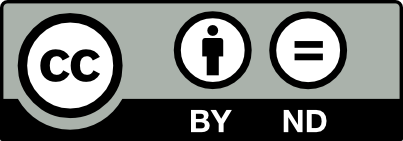
\includegraphics[width=0.3\textwidth]{images/by-nd.png}
    \caption{Attribution CC BY-ND}
    \label{fig:ccBYND}
    \end{figure}


    \item Attribution - Non-commercial (CC BY-NC).

    \begin{figure}[H]
    \centering
    
\includegraphics[width=0.3\textwidth]{images/by-nc.png}
    \caption{Attribution CC BY-NC}
    \label{fig:ccBYNC}
    \end{figure}
 \end{itemize}
 
The following license differs from the aforementioned types since it forbids the production of derivative works. Thus, adaptations are not allowed, but the work can still be used commercially (as long as credit is given to the author).

\begin{itemize} 
  \item Attribution - Non-commercial - Share alike (CC BY-NC-SA)

    \begin{figure}[H]
    \centering
    
\includegraphics[width=0.3\textwidth]{images/by-nc-sa.png}
    \caption{Attribution CC BY-NC-SA}
    \label{fig:ccBYNCSA}
    \end{figure}
\end{itemize}

Similarly to the above CC BY-NC-SA license, the following one works exactly the same, with the exception that it does not allow for the commercial reuse.

\begin{itemize} 

  \item Attribution - Non-commercial - No derivative works (CC BY-NC-ND)

    \begin{figure}[H]
    \centering
    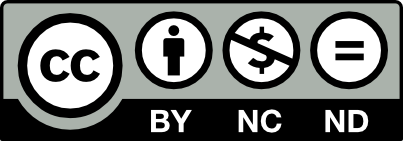
\includegraphics[width=0.3\textwidth]{images/by-nc-nd.png}
    \caption{Attribution CC BY-NC-ND}
    \label{fig:ccBYNCND}
    \end{figure}

\end{itemize}

Finally, another tool called “Public Domain Dedication” or “CC0” allows for waiving all the related rights and effectively put the work into the worldwide public domain.

    \begin{figure}[H]
    \centering
    
\includegraphics[width=0.3\textwidth]{images/cc-zero.png}
    \caption{Public Domain Dedication}
    \label{fig:cc0}
    \end{figure}

“CC0 allows reusers to distribute, remix, adapt, and build upon the material in any medium or format, with no conditions.”\footfullcite{cc0}

The CC licenses do not contain specific terms about the distribution of source code because they are mainly focused on writings, visual arts, and other creative works. Alternative forms of permissive licensing specifically made for software production also exist. One source containing the range of licenses that are around is: “Various Licenses and Comments About Them”\footfullcite{gnuLicenses} by the Free Software Foundation which provides a list of software licenses with explanations.

By combining the Open Source and Creative Commons the Remix Culture can thrive with new works of creativity which are perfectly legal. An ideal solution would be to propagate the ideas and an understanding of the Creative Commons licenses to encourage their usage among all levels of actors hoping that the openness will create a virtuous cycle that benefits everyone involved.